\documentclass[11pt,a4paper]{article}

\usepackage[margin=2.5cm]{geometry}
\usepackage{amsmath,amssymb}
\usepackage{bm}
\usepackage{graphicx}
\usepackage{booktabs}
\usepackage{xcolor}
\usepackage[colorlinks=true,linkcolor=blue!60!black,urlcolor=blue!60!black]{hyperref}
\usepackage{cleveref}
\usepackage[section]{placeins}

% All parameters and quoted numbers, written by figures/plot_impurity.py from figures/configs_spin_chain/*.nml.
% Written by figures/plot_impurity.py from figures/configs_spin_chain/*.nml; do not edit.
\newcommand{\nq}{10}
\newcommand{\jval}{5}
\newcommand{\epsval}{2}
\newcommand{\hval}{0.1}
\newcommand{\kval}{20}
\newcommand{\tr}{30}
\newcommand{\trtwo}{60}
\newcommand{\impseed}{12345}
\newcommand{\initpol}{z}
\newcommand{\initsign}{+}
\newcommand{\ntheta}{100}
\newcommand{\nphi}{200}
\newcommand{\nruns}{3}
\newcommand{\deltazA}{0}
\newcommand{\deltaxA}{0}
\newcommand{\FtrA}{0.885}
\newcommand{\FendA}{1}
\newcommand{\FdefA}{4.3\times10^{-14}}
\newcommand{\Qzero}{0.9995}
\newcommand{\QtrA}{1}
\newcommand{\QendA}{1}
\newcommand{\deltazB}{0.05}
\newcommand{\deltaxB}{0.05}
\newcommand{\FtrB}{0.925}
\newcommand{\FendB}{0.933}
\newcommand{\FdefB}{6.7\times10^{-2}}
\newcommand{\QtrB}{0.964}
\newcommand{\QendB}{0.954}
\newcommand{\deltazC}{0.5}
\newcommand{\deltaxC}{0.5}
\newcommand{\FtrC}{0.309}
\newcommand{\FendC}{0.159}
\newcommand{\FdefC}{8.4\times10^{-1}}
\newcommand{\QtrC}{0.416}
\newcommand{\QendC}{0.282}
\newcommand{\runrows}{%
  \deltazA & \deltaxA & \FtrA & \FendA & $\FdefA$ & \QtrA & \QendA \\
  \deltazB & \deltaxB & \FtrB & \FendB & $\FdefB$ & \QtrB & \QendB \\
  \deltazC & \deltaxC & \FtrC & \FendC & $\FdefC$ & \QtrC & \QendC \\
}

\newcommand{\widths}{$(\delta_z,\delta_x)=(\deltazA,\deltaxA)$, $(\deltazB,\deltaxB)$ and $(\deltazC,\deltaxC)$}

\title{The Qubit Chain with a Static Impurity\\[0.3em]
  \large Time reversal with random couplings and kicks}
\author{}
\date{}

\begin{document}
\maketitle

\begin{abstract}
The kicked top of spin $j=n_q/2$ is realised by a chain of $n_q$ qubits with an all-to-all Ising coupling and a
kick that rotates every qubit about $x$. A static impurity adds a random offset to every coupling and to every kick
angle. It is drawn once and is the same before and after the time reversal at $t_r$, so the backward evolution no
longer undoes the forward one. The echo is compared for \nruns{} impurity widths and two initial spin coherent states through the fidelity,
the total spin and the Husimi distribution. Without impurity, the butterfly effect is shown by rotating one qubit at
$t_r$ by \nalpha{} angles about $x$, $y$ and $z$.
\end{abstract}

%=====================================================================
\section{Model}\label{sec:model}
%=====================================================================

The clean chain has the Floquet operator
\begin{equation}\label{eq:U0}
  U_0 = e^{-i\varepsilon H_{zz}}\prod_{i=1}^{n_q} e^{-i\frac{h}{2}\sigma^x_i},\qquad
  H_{zz} = \frac14\sum_{i,l=1}^{n_q}\sigma^z_i\sigma^z_l,
\end{equation}
so that $H_{zz}=S_z^2$ and $\prod_i e^{-i\frac h2\sigma^x_i}=e^{-ihS_x}$ with $\bm S=\frac12\sum_i\bm\sigma_i$.
The static impurity has two parts:
\begin{equation}\label{eq:imp}
  H_\xi = \sum_{i,l=1}^{n_q}\xi_{il}\,\sigma^z_i\sigma^z_l,\qquad
  \xi_{il}=\xi_{li}\in\left[-\tfrac{\delta_z}{2},\tfrac{\delta_z}{2}\right]\ (i<l),\quad \xi_{ii}=0,
\end{equation}
an offset of every pair coupling, and an offset $\mu_i\in[-\frac{\delta_x}{2},\frac{\delta_x}{2}]$ of the kick
angle of qubit $i$. All $\xi_{il}$ and $\mu_i$ are independent and uniformly distributed, drawn once from the seed
\texttt{imp\_seed} and then kept fixed. One forward step is
\begin{equation}\label{eq:U}
  U = e^{-i(\varepsilon H_{zz}+H_\xi)}\prod_{i=1}^{n_q} e^{-i\frac{h+\mu_i}{2}\sigma^x_i}.
\end{equation}

\paragraph{Time reversal.}
After $t_r$ forward steps the controllable parameters are reversed, $\varepsilon\to2\pi-\varepsilon$ and $h\to-h$, but
the impurity is not: it keeps its values and its sign. One backward step is
\begin{equation}\label{eq:Ub}
  U_r = \prod_{i=1}^{n_q} e^{-i\frac{-h+\mu_i}{2}\sigma^x_i}\,e^{-i((2\pi-\varepsilon)H_{zz}+H_\xi)},
  \qquad \psi(t) = U_r^{\,t-t_r}U^{t_r}\psi(0),\quad t_r<t\le2t_r .
\end{equation}
For $\delta_z=\delta_x=0$, $e^{-2\pi iH_{zz}}=e^{-2\pi iS_z^2}$ is a global phase and $U_r=U^{-1}$, so
$\psi(2t_r)=\psi(0)$ up to a phase. With the impurity, the clean parts still cancel in $U_rU$ but the impurity
parts add up: the coupling term gives $e^{-2iH_\xi}$, and the kick angles $\pm h+\mu_i$ no longer cancel.
The echo is measured by the fidelity
\begin{equation}\label{eq:F}
  F(t) = |\langle\psi(0)|\psi(t)\rangle|^2 .
\end{equation}

\paragraph{Butterfly effect.}
In the butterfly runs there is no impurity, and qubit $i=\iflip$ is rotated about $a=x,y,z$ by an angle $\alpha$ at
$t_r$, before the backward leg:
\begin{equation}\label{eq:bf}
  \psi(t) = U^{-(t-t_r)}R\,U^{t_r}\psi(0),\qquad R=e^{-i\frac\alpha2\sigma^a_i},\quad t_r<t\le2t_r .
\end{equation}

%=====================================================================
\section{Parameters}\label{sec:parameters}
%=====================================================================

The chain has $n_q=\nq$ qubits ($j=\jval$), coupling $\varepsilon=\epsval$ (classical torsion $k=n_q\varepsilon=\kval$)
and kick angle $h=\hval$. Every qubit starts in the same spin-$\frac12$ coherent state $|\theta_0,\phi_0\rangle$, so
$\psi(0)=|\theta_0,\phi_0\rangle^{\otimes n_q}$ is the spin coherent state $|\theta_0,\phi_0\rangle$ of the top, with
$\langle\bm S\rangle/j=(\sin\theta_0\cos\phi_0,\sin\theta_0\sin\phi_0,\cos\theta_0)$ and its Husimi distribution
centred at $(\theta_0,\phi_0)$. Two initial states are compared, $(\theta_0,\phi_0)=(\thetaOne,\phiOne)$ and
$(\thetaTwo,\phiTwo)$; every figure is shown for both. Each is evolved for
$t_r=\tr$ forward and $t_r$ backward steps. The butterfly runs are in \cref{sec:butterfly}; the impurity runs
have no qubit rotation at $t_r$. The Husimi distribution is evaluated on $\ntheta\times\nphi$ points in $(Z,\phi)$.

%=====================================================================
\section{Butterfly effect}\label{sec:butterfly}
%=====================================================================

\Cref{fig:butterfly_x,fig:butterfly_y,fig:butterfly_z} show $F(t)$ without impurity when qubit \iflip{} is rotated at
$t_r$ by $\alpha=\alphaA,\alphaB,\alphaC,\alphaD,\alphaE$ about $x$, $y$ and $z$, \cref{eq:bf}, one line per
angle. For $t\le t_r$ all curves are those of the clean chain.

\begin{figure}[ht]
  \centering
  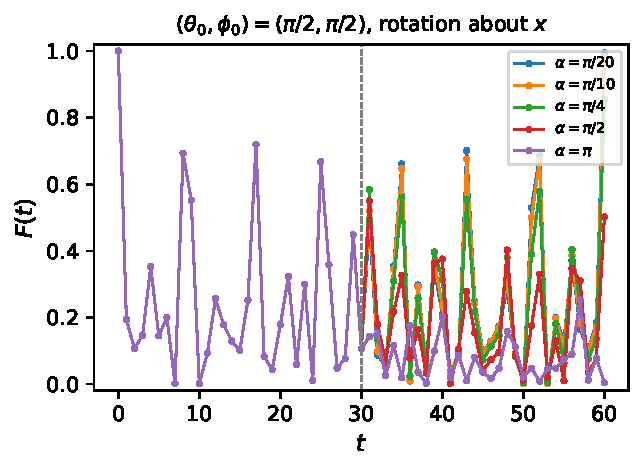
\includegraphics[width=0.49\textwidth]{figures/impurity_butterfly_x_One.pdf}\hfill
  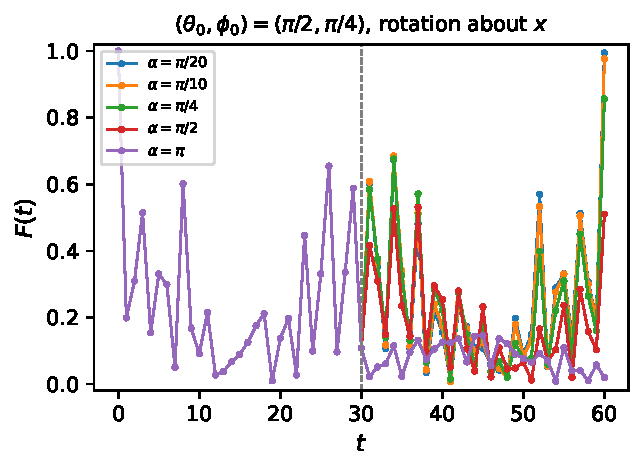
\includegraphics[width=0.49\textwidth]{figures/impurity_butterfly_x_Two.pdf}
  \caption{Fidelity $F(t)$ without impurity, qubit \iflip{} rotated about $x$ by $\alpha$ at $t_r=\tr$ (dashed).
    Left: $(\theta_0,\phi_0)=(\thetaOne,\phiOne)$, right: $(\thetaTwo,\phiTwo)$.}
  \label{fig:butterfly_x}
\end{figure}

\begin{figure}[ht]
  \centering
  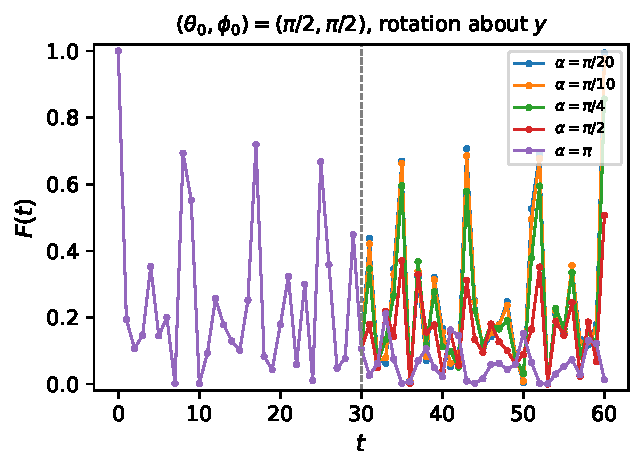
\includegraphics[width=0.49\textwidth]{figures/impurity_butterfly_y_One.pdf}\hfill
  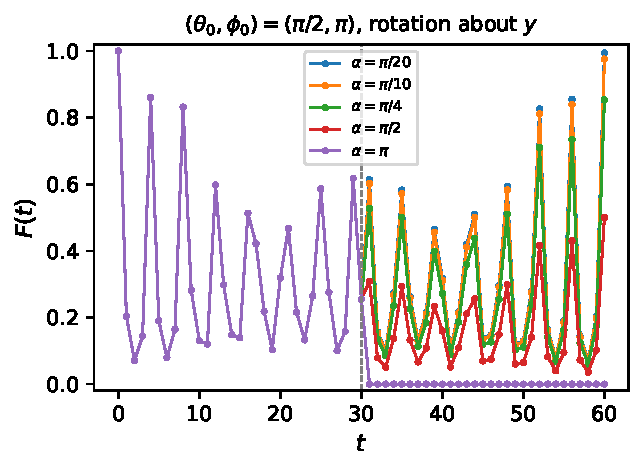
\includegraphics[width=0.49\textwidth]{figures/impurity_butterfly_y_Two.pdf}
  \caption{Fidelity $F(t)$ without impurity, qubit \iflip{} rotated about $y$ by $\alpha$ at $t_r=\tr$ (dashed).
    Left: $(\theta_0,\phi_0)=(\thetaOne,\phiOne)$, right: $(\thetaTwo,\phiTwo)$.}
  \label{fig:butterfly_y}
\end{figure}

\begin{figure}[ht]
  \centering
  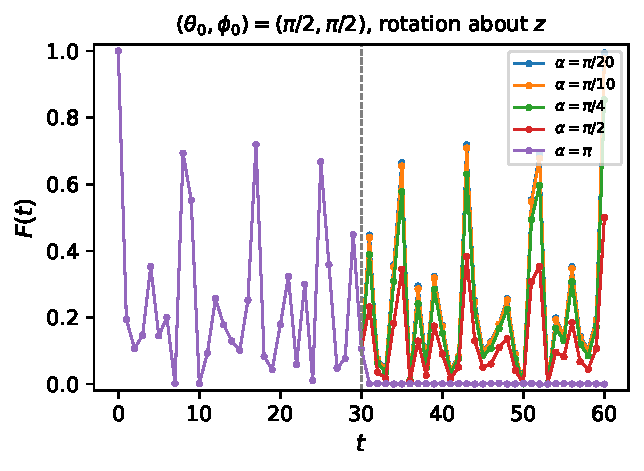
\includegraphics[width=0.49\textwidth]{figures/impurity_butterfly_z_One.pdf}\hfill
  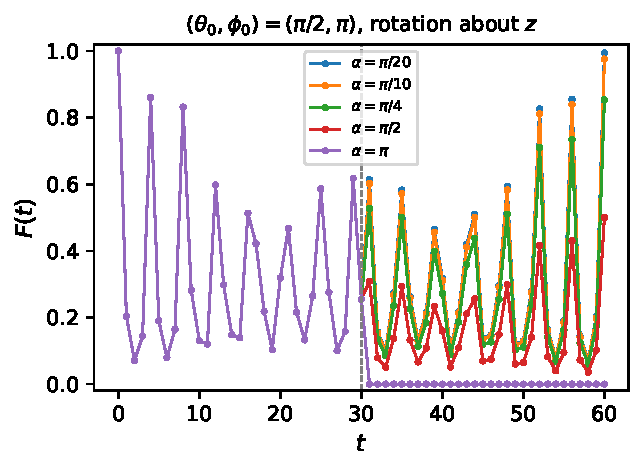
\includegraphics[width=0.49\textwidth]{figures/impurity_butterfly_z_Two.pdf}
  \caption{Fidelity $F(t)$ without impurity, qubit \iflip{} rotated about $z$ by $\alpha$ at $t_r=\tr$ (dashed).
    Left: $(\theta_0,\phi_0)=(\thetaOne,\phiOne)$, right: $(\thetaTwo,\phiTwo)$.}
  \label{fig:butterfly_z}
\end{figure}

%=====================================================================
\section{Fidelity}\label{sec:fidelity}
%=====================================================================

\Cref{fig:fidelity} shows $F(t)$ for all runs. Without impurity the backward leg retraces the forward one,
$F(t_r+s)=F(t_r-s)$, and the echo is exact to rounding, $|1-F(2t_r)|=\FdefAOne$ and $\FdefATwo$ for the two
initial states. With the impurity the forward evolution itself changes, and the backward leg does not return to
$\psi(0)$. For $(\theta_0,\phi_0)=(\thetaOne,\phiOne)$, $F(2t_r)=\FendBOne$ for $\delta_z=\deltazB$,
$\delta_x=\deltaxB$ and $F(2t_r)=\FendCOne$ for $\delta_z=\deltazC$, $\delta_x=\deltaxC$. For
$(\thetaTwo,\phiTwo)$ the same impurities give $F(2t_r)=\FendBTwo$ and $\FendCTwo$.

\begin{figure}[ht]
  \centering
  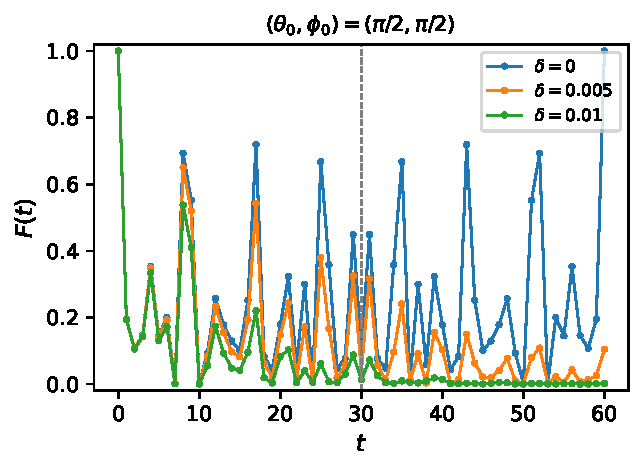
\includegraphics[width=0.49\textwidth]{figures/impurity_fidelity_One.pdf}\hfill
  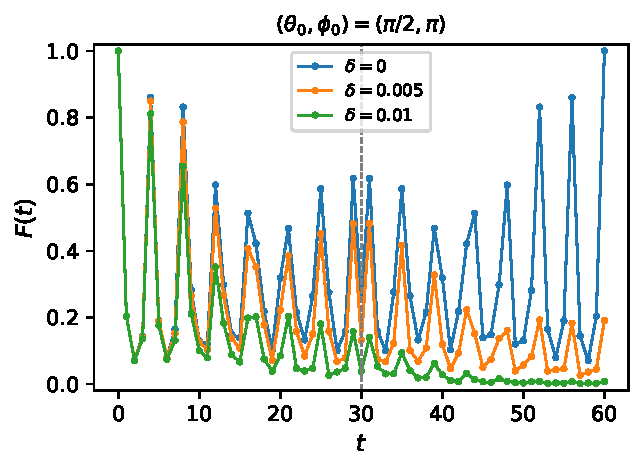
\includegraphics[width=0.49\textwidth]{figures/impurity_fidelity_Two.pdf}
  \caption{Fidelity $F(t)$, \cref{eq:F}, for the impurity widths \widths. Left:
    $(\theta_0,\phi_0)=(\thetaOne,\phiOne)$, right: $(\thetaTwo,\phiTwo)$. Dashed: the reversal $t_r=\tr$.}
  \label{fig:fidelity}
\end{figure}

%=====================================================================
\section{Total spin}\label{sec:spin}
%=====================================================================

\Cref{fig:S_a,fig:J2_a} show the components $\langle S_a\rangle/j$ and $\langle S_a^2\rangle/j^2$, $a=x,y,z$, of the
total spin, one figure per component. For $\delta_z=\delta_x=0$ each curve is symmetric about $t_r$ and returns to
its initial value at $2t_r$; with the impurity it does not. The clean chain conserves $\bm S^2=j(j+1)$. The random
couplings and kick angles differ from qubit to qubit and break the permutation symmetry, so with the impurity
$\langle\bm S^2\rangle$ is no longer conserved, and $\sum_a\langle S_a^2\rangle/j^2$ is not fixed.

\begin{figure}[p]
  \centering
  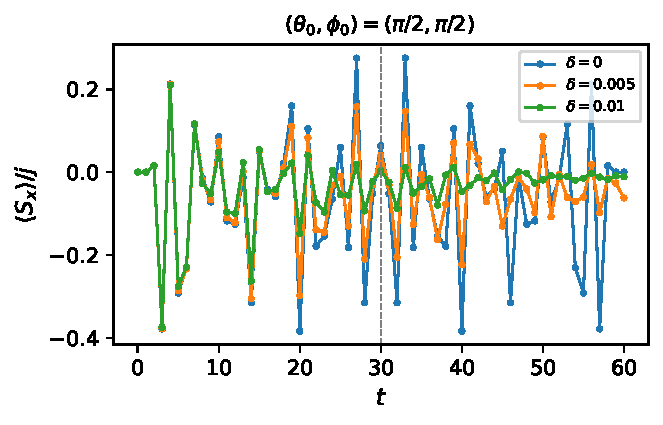
\includegraphics[width=0.49\textwidth]{figures/impurity_Jx_One.pdf}\hfill
  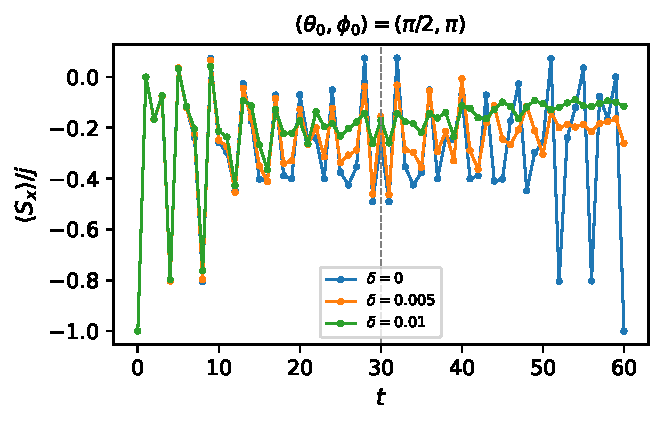
\includegraphics[width=0.49\textwidth]{figures/impurity_Jx_Two.pdf}\\[0.5em]
  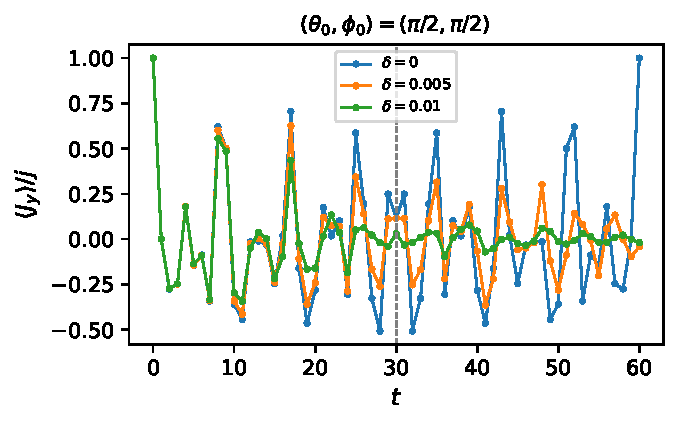
\includegraphics[width=0.49\textwidth]{figures/impurity_Jy_One.pdf}\hfill
  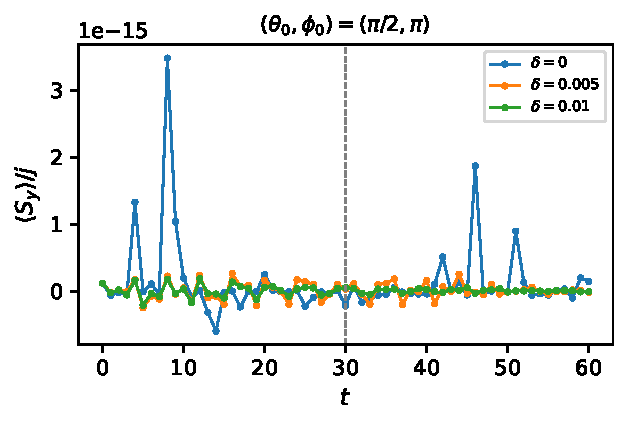
\includegraphics[width=0.49\textwidth]{figures/impurity_Jy_Two.pdf}\\[0.5em]
  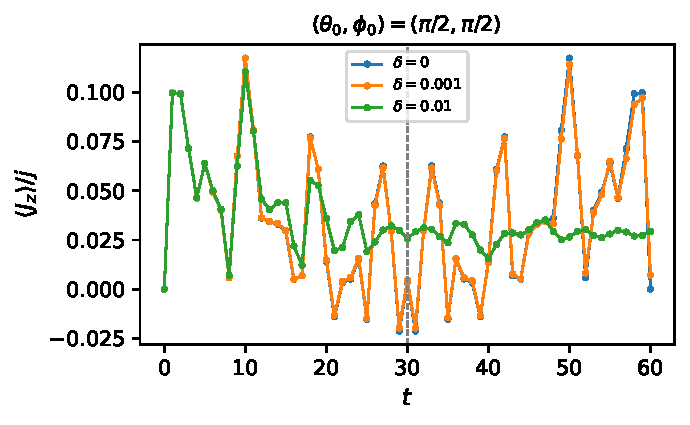
\includegraphics[width=0.49\textwidth]{figures/impurity_Jz_One.pdf}\hfill
  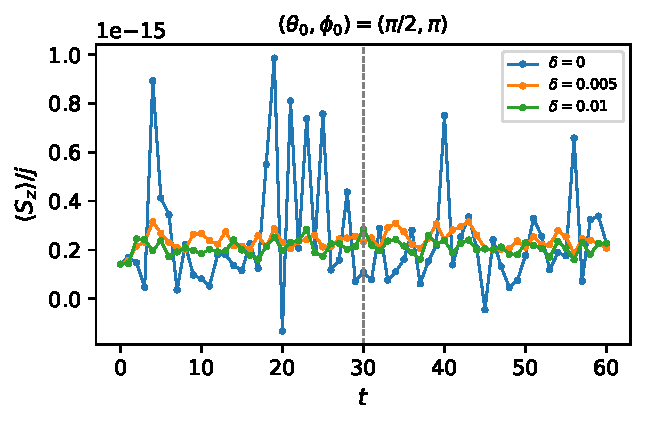
\includegraphics[width=0.49\textwidth]{figures/impurity_Jz_Two.pdf}
  \caption{$\langle S_x\rangle/j$ (top), $\langle S_y\rangle/j$ (middle) and $\langle S_z\rangle/j$ (bottom) for the
    impurity widths \widths. Left: $(\theta_0,\phi_0)=(\thetaOne,\phiOne)$, right: $(\thetaTwo,\phiTwo)$.
    Dashed: $t_r$.}
  \label{fig:S_a}
\end{figure}

\begin{figure}[p]
  \centering
  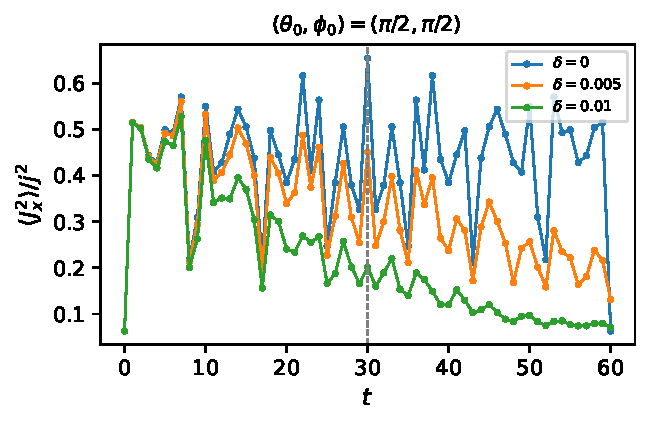
\includegraphics[width=0.49\textwidth]{figures/impurity_J2x_One.pdf}\hfill
  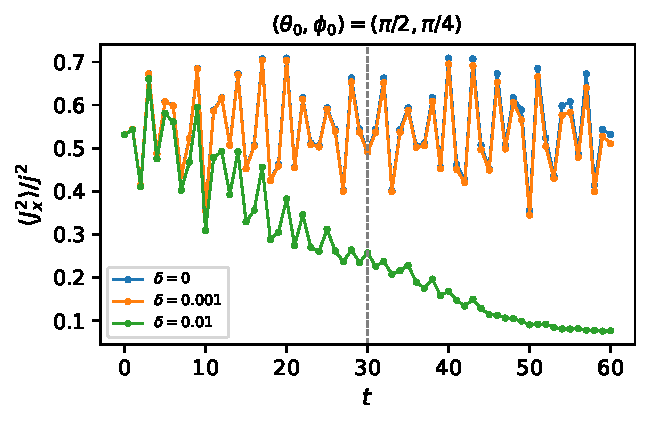
\includegraphics[width=0.49\textwidth]{figures/impurity_J2x_Two.pdf}\\[0.5em]
  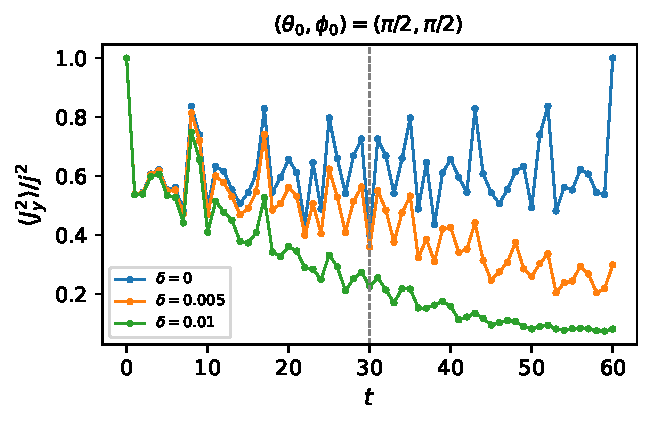
\includegraphics[width=0.49\textwidth]{figures/impurity_J2y_One.pdf}\hfill
  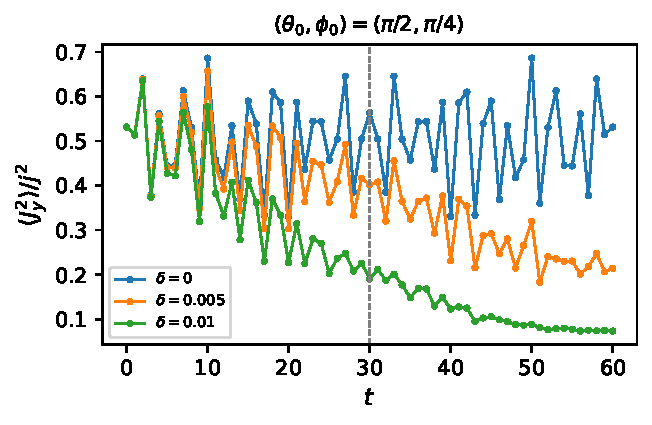
\includegraphics[width=0.49\textwidth]{figures/impurity_J2y_Two.pdf}\\[0.5em]
  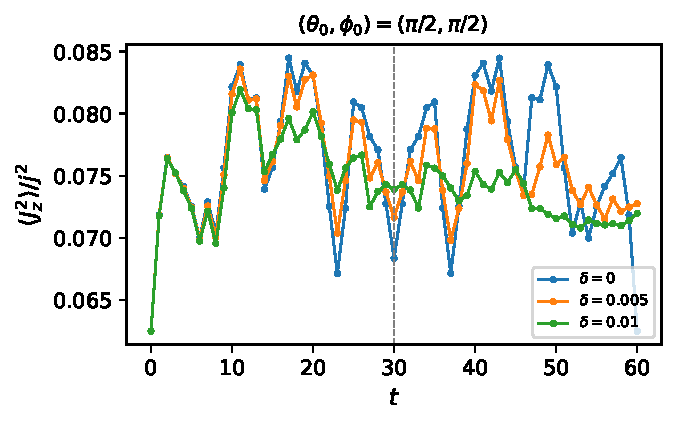
\includegraphics[width=0.49\textwidth]{figures/impurity_J2z_One.pdf}\hfill
  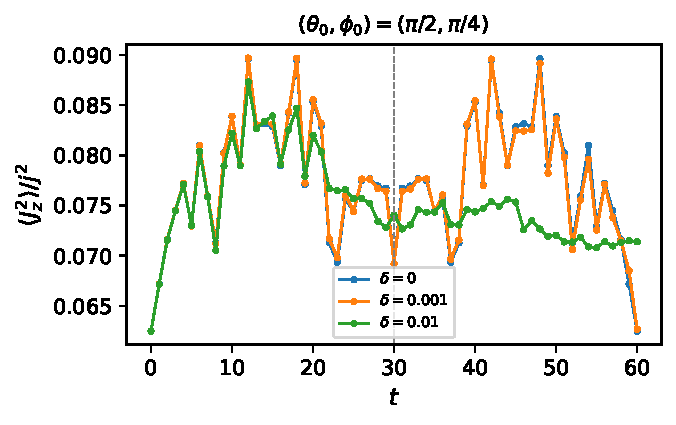
\includegraphics[width=0.49\textwidth]{figures/impurity_J2z_Two.pdf}
  \caption{$\langle S_x^2\rangle/j^2$ (top), $\langle S_y^2\rangle/j^2$ (middle) and $\langle S_z^2\rangle/j^2$
    (bottom) for the impurity widths \widths. Left: $(\theta_0,\phi_0)=(\thetaOne,\phiOne)$, right:
    $(\thetaTwo,\phiTwo)$. Dashed: $t_r$.}
  \label{fig:J2_a}
\end{figure}

%=====================================================================
\section{Husimi distribution}\label{sec:husimi}
%=====================================================================

\Cref{fig:husimiOne,fig:husimiTwo} show the Husimi distribution $Q(\theta,\phi)=|\langle\theta,\phi|\psi(t)\rangle|^2$
of the chain state, at $t=0$, $t_r$ and $2t_r$, one row per impurity width, for the two initial states. At $t=0$ it
is centred at $(\theta_0,\phi_0)$, i.e.\ at $Z=\cos\theta_0$ and $\phi=\phi_0$. Without impurity the distribution at
$2t_r$ equals the initial one. The spin coherent states $|\theta,\phi\rangle$ lie in the symmetric (Dicke) subspace $j=n_q/2$, so
$Q$ only sees the projection of $\psi(t)$ onto it. The clean chain never leaves this subspace; the impurity breaks
the permutation symmetry and moves weight out of it. The Husimi norm
\begin{equation}\label{eq:QN}
  \mathcal N(t) = \frac{2j+1}{4\pi}\int Q\,dZ\,d\phi
\end{equation}
is the symmetric weight of $\psi(t)$, up to the quadrature error of the grid ($\mathcal N(0)=\Qzero$ for the
normalised initial state).

\begin{figure}[ht]
  \centering
  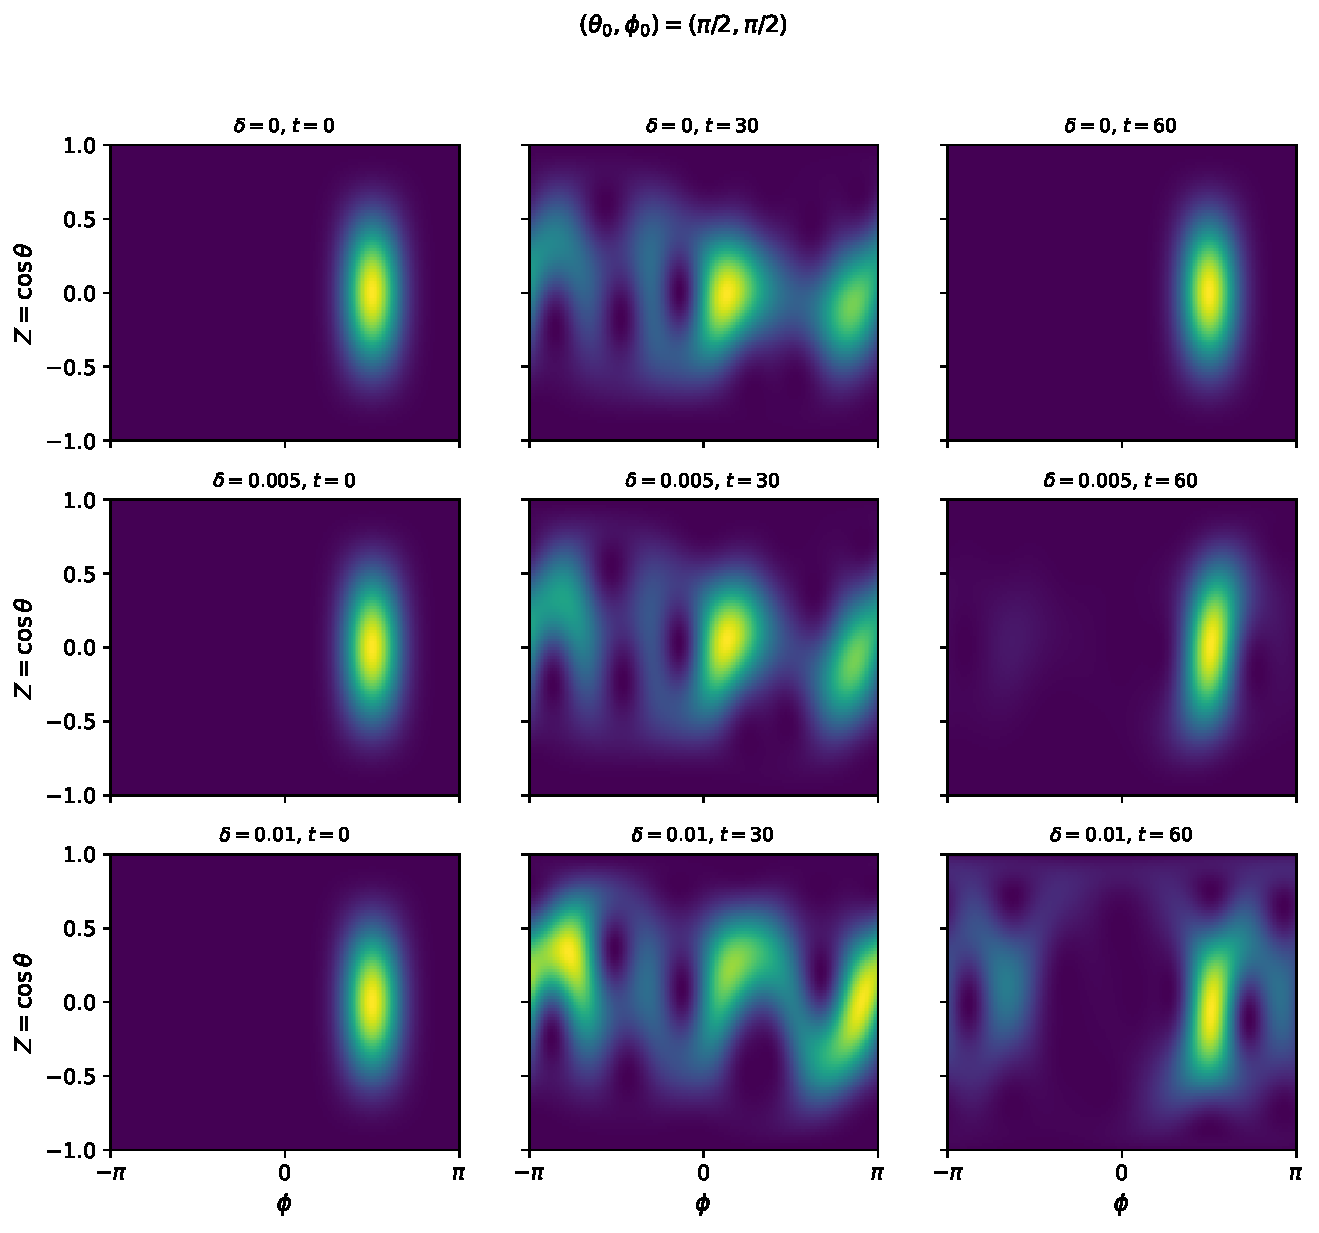
\includegraphics[width=\textwidth]{figures/impurity_husimi_One.pdf}
  \caption{Husimi distribution for $(\theta_0,\phi_0)=(\thetaOne,\phiOne)$ at $t=0$ (left), $t_r=\tr$ (middle) and
    $2t_r=\trtwo$ (right). Rows: the impurity widths \widths. Each panel has its own colour scale.}
  \label{fig:husimiOne}
\end{figure}

\begin{figure}[ht]
  \centering
  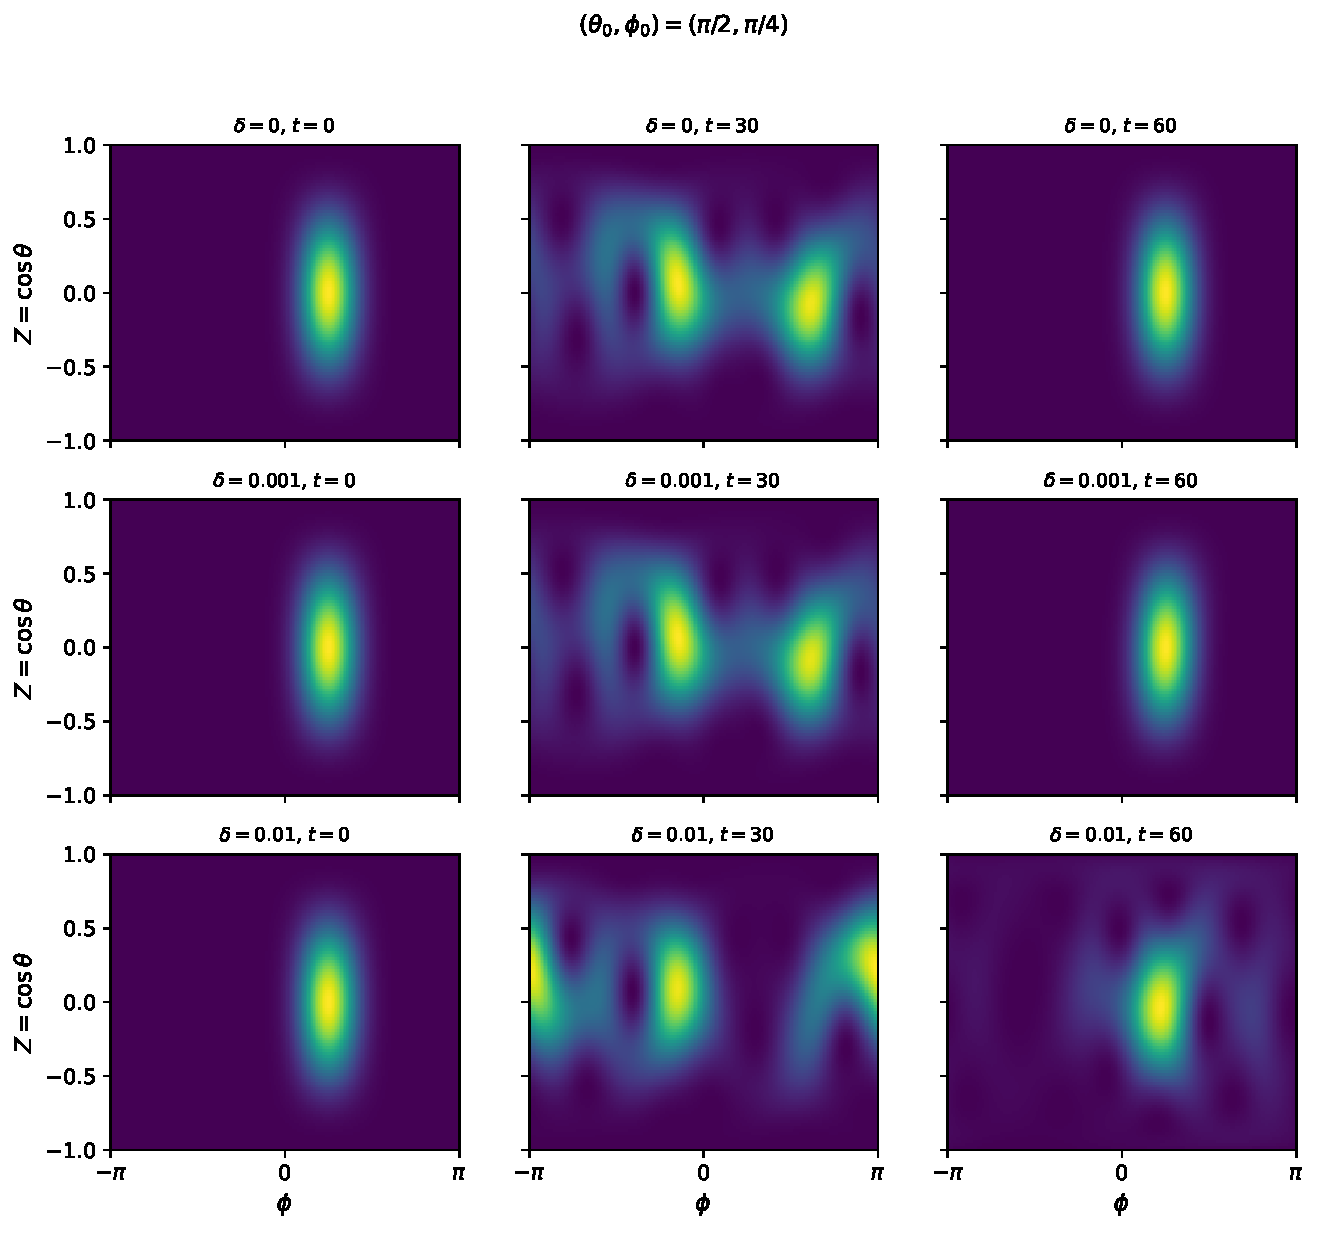
\includegraphics[width=\textwidth]{figures/impurity_husimi_Two.pdf}
  \caption{As \cref{fig:husimiOne}, for $(\theta_0,\phi_0)=(\thetaTwo,\phiTwo)$.}
  \label{fig:husimiTwo}
\end{figure}

%=====================================================================
\section{Notation}\label{sec:notation}
%=====================================================================

\begin{itemize}
  \item $n_q$: number of qubits; $j=n_q/2$: spin of the top.
  \item $i,l=1,\dots,n_q$: qubit indices.
  \item $\sigma^a_i$, $a=x,y,z$: Pauli matrix $a$ of qubit $i$; $\bm\sigma_i=(\sigma^x_i,\sigma^y_i,\sigma^z_i)$.
  \item $\bm S=\frac12\sum_i\bm\sigma_i$, $S_a$: total spin and its component $a$; $\bm S^2$: its square.
  \item $\langle\cdot\rangle$: expectation value in $\psi(t)$.
  \item $H_{zz}$: all-to-all Ising coupling, \cref{eq:U0}.
  \item $\varepsilon$: coupling strength; $k=n_q\varepsilon$: classical torsion.
  \item $h$: kick angle about $x$.
  \item $U_0$, $U$: clean and impure forward Floquet operators, \cref{eq:U0,eq:U}; $U_r$: backward Floquet
    operator, \cref{eq:Ub}.
  \item $H_\xi$, $\xi_{il}$: impurity of the couplings, \cref{eq:imp}; $\delta_z$: width of the $\xi_{il}$.
  \item $\mu_i$: impurity of the kick angle of qubit $i$; $\delta_x$: width of the $\mu_i$.
  \item \texttt{imp\_seed}: seed of the random numbers $\xi_{il}$, $\mu_i$.
  \item $t$: number of kicks (time); $t_r$: time of the reversal; $2t_r$: end of the echo.
  \item $\psi(t)$: state of the chain at time $t$.
  \item $(\theta,\phi)$: polar and azimuthal angle on the unit sphere; $Z=\cos\theta$.
  \item $|\theta,\phi\rangle$: spin coherent state; $(\theta_0,\phi_0)$: direction of the initial state.
  \item $F(t)$: fidelity, \cref{eq:F}.
  \item $R$: rotation of qubit $i$ at $t_r$ in the butterfly runs, \cref{eq:bf}; $a$: its axis; $\alpha$: its angle.
  \item $Q(\theta,\phi)$: Husimi distribution; $\mathcal N(t)$: Husimi norm, \cref{eq:QN}.
\end{itemize}

\end{document}
